\documentclass{article}
\usepackage[usenames,dvipsnames]{color}
\usepackage{appendix}
\usepackage{authblk}
\usepackage{amsmath}
\usepackage{mathtools}
\usepackage{amsthm}
\usepackage{caption}
\usepackage{subcaption}
\usepackage[utf8]{inputenc}
\usepackage{hyperref}
\hypersetup{
 colorlinks=true,
 linkcolor = black,
 citecolor = black}
\usepackage[
backend=biber,
style=alphabetic,
sorting=ynt
]{biblatex}
\addbibresource{biblio.bib}

\theoremstyle{definition}
\newtheorem{exmp}{Example}

\captionsetup[figure]{labelfont={bf},name={Fig.},labelsep=period}

\pagestyle{plain}

\title{\vspace{-1.0cm}Fluidity Money: Economics and Monetary Policy}
\author[]{Erik Brauer}
\author[]{Shahmeer Chaudhry}
\author[]{Alexander Baigent}
\affil[]{Fluidity Money}
\date{October 2021} 

\begin{document}

\maketitle

\begin{abstract}
    Fluidity Money tokens (Fluid Assets) are a 1-to-1 wrapped asset that exposes holders to randomly paid large dividend rewards. Dividends are paid out according to a drawing mechanism held on each transaction of their Fluid Assets. Dividends are generated by the cumulative yield created by every principal token deposited and lent on money markets.
\end{abstract}


\section{Introduction}

Existing decentralised finance incentivises leaving interest-bearing products "idle" -- sitting in an account accruing interest. The majority of the world's population lives paycheck-to-paycheck and cannot afford to leave their money in an inaccessible account. This demographic is unable to lift itself out of poverty on the back of these instruments and is unable to participate in the financial system beyond simple banking.

Fluid Assets expose this demographic to decentralised finance. Fluidity Money's reward pool and yield generation mechanism operates similarly to a "no-loss lottery", pioneered by existing products, including PoolTogether \cite{pool}. Users exchange principal tokens into 1-to-1 backed Fluid Assets and that money is then lent on a yield-generating protocol. This cumulative yield makes up the reward pool that users are exposed to on each transfer of their wrapped (Fluid Asset) token. This reward mechanism incentivises taking Fluid Assets over their non-Fluid equivalent, as Fluid Assets can always be redeemed for their principal at no cost.

The system is modelled to be sound using the unique design of the Transfer Reward Function. Governance tokens are distributed through the use of a novel approach similar to liquidity mining titled Utility Mining. This unique approach to provisioning tokens incentivises adoption of the platform through the provision of liquidity. In the future, Fluidity will support guaranteed future yield by facilitating the sale of expected outcomes, similarly to Alchemix \cite{alchemix} and Pendle \cite{pendle}.

Fluidity Money's design necessitates careful and well-intentioned economics modelling. The platform should be resilient enough to withstand abuse from malicious actors while providing enough utility to be deemed useful. We examine Fluidity's design in the following.

\newpage

\section{Cyclic Transaction Attack}

To mitigate abuse of the system, we investigate different attack vectors and how to dampen their effects on the overall integrity of the protocol. 

Consider a risk neutral adversary sending funds in a periodic or random pattern with the goal of increasing their chances of receiving dividends by cheating the system. We explore different strategies to mitigate this attack, one of which we will highlight in the following section.

\subsection{Optimistic Solution}

We can calculate the expected yield after $n$ transactions of an adversary trying to attack the system with a sybil-like or cyclical transaction pattern as follows:

\begin{equation}
    \frac{\textsc{gain}-\textsc{loss}}{S_0} = \textsc{yield},
\end{equation}

where $S_0$ is the starting capital and $\textsc{gain}(w,p)$ is a function of the payouts and the associated probabilities, which describes the expected gains with \cite{feller}

\begin{equation}
    \textsc{gain} = n \cdot \mu = n \sum_{m=1}^M w_m p_m,
\end{equation}

where $n$ is the number of transactions and $M$ describes the number of divisions or "dividend tiers". $\textsc{loss}$ can be derived recursively as follows:

\begin{equation}
    \textsc{loss} = S_0-S_n = 
    \begin{dcases} 
      n \cdot g & f = 0 \\
      \frac{1}{f}(g+fS_0-fg)(1-(1-f)^n) & f > 0 \\
    \end{dcases},
\end{equation}

where 

\begin{equation}
    S_n = (S_{n-1}-g)(1-f), \: S_n > 0.
\end{equation}

$g$ is the associated gas fee and $f$ is an extra dynamic fee that is deducted after the static gas fee (e.g. the liquidity provider fee on AMMs like Uniswap). It is reasonable to suppose that an attacker will always choose platforms with the lowest fees, i.e. without dynamic fees, henceforth we will assume the worst-case scenario where $f=0$.

The objective of the optimistic solution is to keep the expected yield of an attacker below a certain percentage, which we can achieve by setting $\mu \leq g$ for every transaction. To obtain the vector $w_m$, we find a payout function that returns the payouts for a given reward pool, divisions and protocol parameters and that satisfies the aforementioned condition for the expected value. We derive this function in the following section. 

Finally, in the case of an attacker reusing their rewards, it is trivial to see that their chance of ruin will always be certain if the expected value for every transaction is below or equal to zero, i.e. $\mu \leq g$. \cite{gambler}

\newpage

\section{Transfer Reward Function}

We can derive the Transfer Reward Function (TRF) as a power function with coefficients $a$ and $b$ as follows:

\begin{equation} \label{trf}
    w_m = a\cdot p_m^b = a\cdot p_m^{-1}.
\end{equation}

For $a$, we can evaluate

\begin{equation} \label{trf2}
    a = \frac{1}{M}
    \begin{dcases}
    \frac{\Xi}{ATX} & \mu \leq g \\
    g & \mu > g
    \end{dcases},
\end{equation}

where $M$ is the number of divisions, $\Xi$ is the size of the reward pool, and $ATX$ is the average annual number of transactions. We can see that $\mu = \Xi/ATX$.


A normalized graph of (\ref{trf}) can be seen below in \autoref{fig1}. 

\begin{figure}[hb]
    \centering
    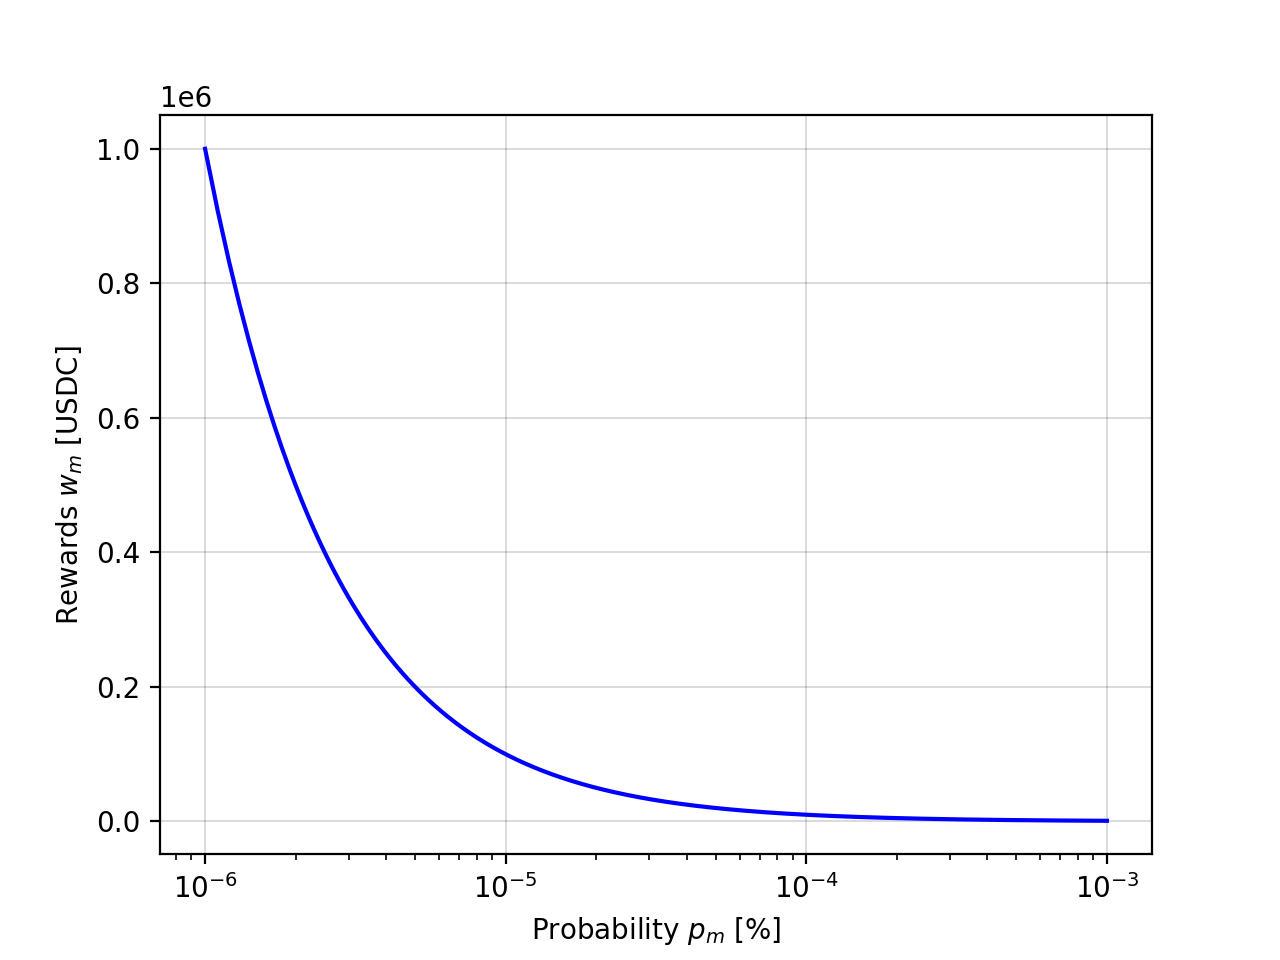
\includegraphics[width=10.5cm]{images/Figure_1.png}
    \caption{Normalized log-plot of the TRF} \label{fig1}
\end{figure}

Observing (\ref{trf2}) in detail shows that for lower volumes the reward payouts will be greater, revealing the TRFs self-regulating property due to variations in utility. As the staked pool increases over time, the rewards grow with it and the protocol will be able to "support" and attract more users.

In the following section we introduce an extension of the TRF with the Elastic Sigmoid Curve, a multiplier coefficient intended to incentivise users to engage more with the protocol by rewarding them based on their behaviour, such as staking LP tokens or locking governance tokens.

\newpage

\section{Elastic Sigmoid Curve}

We evaluate the Elastic Sigmoid Curve (ESC) as follows:

\begin{equation} \label{esc}
    c(r,t) = c_0 + \frac{(K-c_0)t}{r+t}
\end{equation}

where $t$ designates the time, $c_0$ is the initial condition and lower boundary at $t=0$, $K$ is the upper boundary with $\lim_{t \to \infty} c(r,t) = K$, and $r$ is a variable depending on the senders and receivers governance token holdings and how much liquidity they provide. It defines the gradient of the curve. The reward value $c(r,t)$ is added as a multiplier coefficient to the TRF introduced in the previous section. In the future we will add more reward multipliers based on governance decisions, e.g. for the type of transaction and where the transaction occurs.

(7) is modeled after the the law of diminishing returns, with a range from $c_0 \leq c(r,t) \leq K,\: \forall t > 0$. It is designed to keep up utility and liquidity for fluid derivatives and to incentivise users to hold their governance tokens in custody. A normalized graph of (\ref{esc}) can be seen below in \autoref{fig2}.

\begin{figure}[hb]
    \centering
    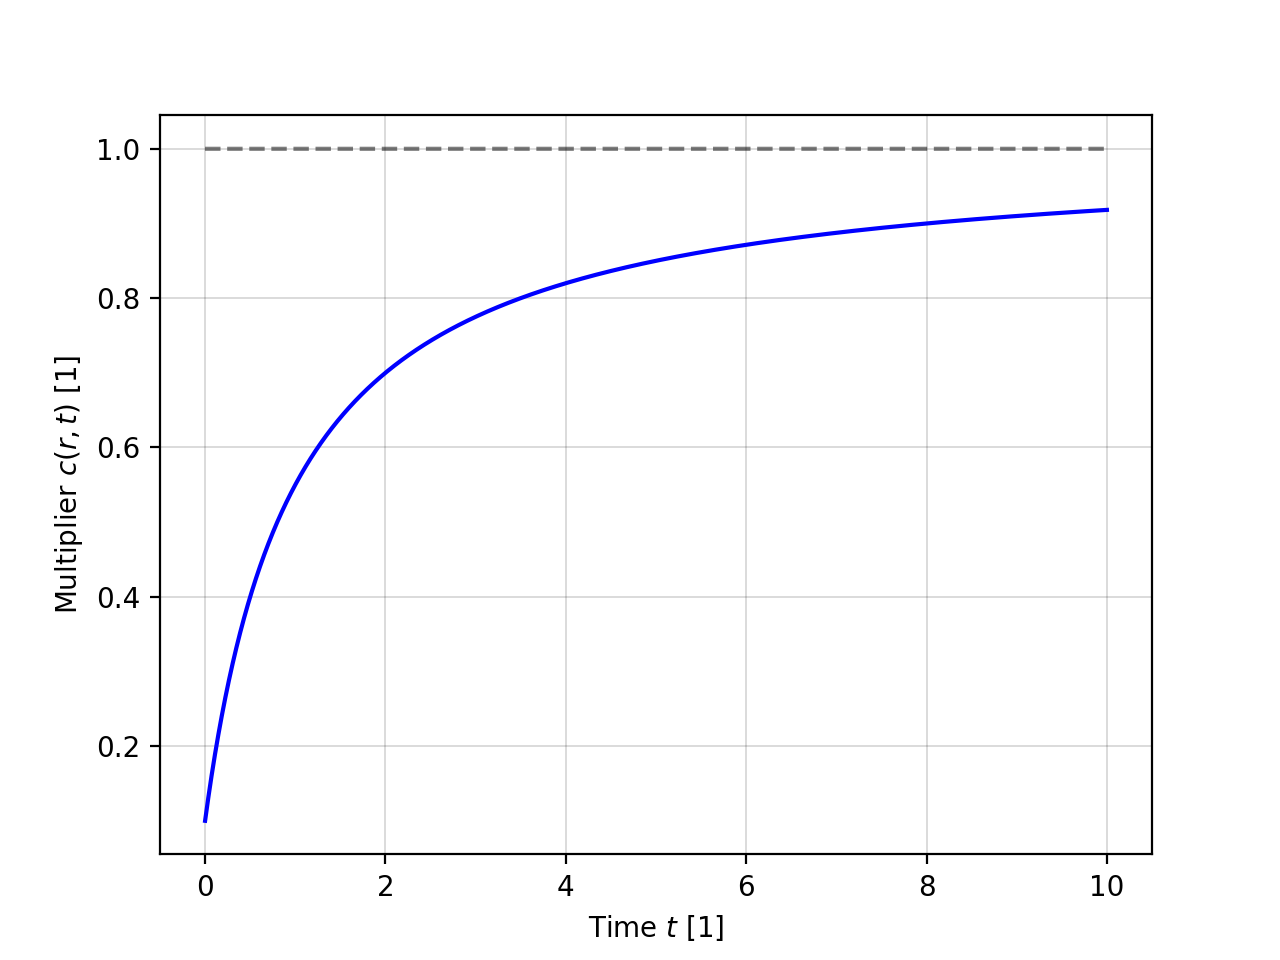
\includegraphics[width=10.5cm]{images/ESCnew.png}
    \caption{Normalized isoline of the ESC, $r=1,\: c_0 = 0.1,\: K=1$} \label{fig2}
\end{figure}

Users will be able to trade and lend their individual rewards on marketplaces ("Outcome Farming"). Once they remove liquidity or unlock their governance tokens, $c(r,t)$ will be reset accordingly based on the percentage of the withdrawn or sold assets. Further design considerations and how to evaluate the reward value $r$ will be discussed in a follow up paper. 

In the next section we introduce Fluidity's drawing mechanism for the dividend system to obtain the probability vector $p_m$.

\newpage

\section{Drawing Mechanism}

The drawing system is comprised by a pool of numbers (balls) that will be randomly chosen for every transaction (ticket) without replacement. We can calculate the chances for $M$ divisions (number of balls in a single ticket for a single transaction) via the hypergeometric distribution as follows \cite{feller}:

\begin{equation}
    p_m = \frac{\binom{M}{m}\binom{N-M}{M-m}}{\binom{N}{M}} = \frac{(M!)^2((N-M)!)^2}{m!N!((M-m)!)^2(m-2M+N)!}
\end{equation}

where $m$ is the number of matching balls for a winning ticket and $N$ is the total number of balls in the pool. To ensure that the largest dividend is paid out at least four times annually, $N$ must satisfy the following condition:

\begin{equation} \label{ncond}
    p_M \geq \frac{4}{ATX} \Leftrightarrow N! < \frac{1}{4} ATX \cdot M! (N-M)!
\end{equation}

A solution to (\ref{ncond}) can be found numerically and may be computed off-chain by finding the largest possible value iteratively or via binary search.

Finally, we can evaluate the TRF in its complete form:

\begin{equation} \label{trff}
    w_m = \frac{1}{M} \Bigg[c_0 + \frac{(K-c_0)t}{t+r}\Bigg] \Bigg(\frac{\binom{M}{m}\binom{N-M}{M-m}}{\binom{N}{M}}\Bigg)^{-1} 
    \begin{dcases}
    \frac{\Xi}{ATX} & \mu \leq g \\
    g & \mu > g
    \end{dcases}
\end{equation}

(\ref{trff}) will be calculated for every single transaction. The value of $M$ may be chosen through governance decisions.

An example table for the payout and probability vectors can be seen below ($\Xi = \$50,000,000$, $ATX = 31,536,000$, $g = \$3$, $M=6$, $c = 1$).

\vspace{1em}
\begingroup
            \centering
            \begin{tabular}{||c | c ||}
            \hline
            $p_m \: [\%]$ & $w_m \: [\$]$ \\[0.5ex]
            \hline
            42.66 & 0.62  \\
            15.69 & 1.69 \\
            2.39 & 11.06 \\
            0.15 & 176.89 \\
            3.23e-3 & 8181.33 \\
            
            1.41e-5 & 1,865,342.25 \\
            \hline
            \end{tabular}
            \par
\endgroup
\vspace{1em}
            

We can see that for $\mu \leq g$

\begin{equation}
    \langle p,w\rangle ATX = \sum_{m=1}^M w_m p_m\cdot ATX = \Xi
\end{equation}

For protocols with smaller fees where $\mu>g$ we explore graph classification models and other strategies in order for them to remain competitive.
We discuss higher expected outcomes through the probability vector $p_m$ by increasing the number of tickets for a single transaction in the aforementioned follow up paper.

\clearpage

To gain a better understanding of how the Transfer Reward Function works together with the Optimistic Solution, we have plotted the isolines for increasing transaction fees in \autoref{fig:fig} on different logarithmic scales. We can see that as the transaction fee increases, the curve of the TRF initally shifts upwards and the rewards for the different tiers increase with it. We can observe that the curve converges towards the equilibrium state of $g \geq \Xi/ATX$. At that point the TRF stops shifting upwards and consequently the magnitude of rewards are dependent on the size of the pool, the total number of fluid transactions and independent of the transaction fee paid by the user. The fee paid by the user thus only affects the payouts when they are low enough, and it doesn't affect the chances of receiving a reward. The same holds true for the ESC and other mechanisms aimed at increasing the expected value for a fluid transaction.


\begin{figure}
\begin{subfigure}{.5\textwidth}
  \centering
  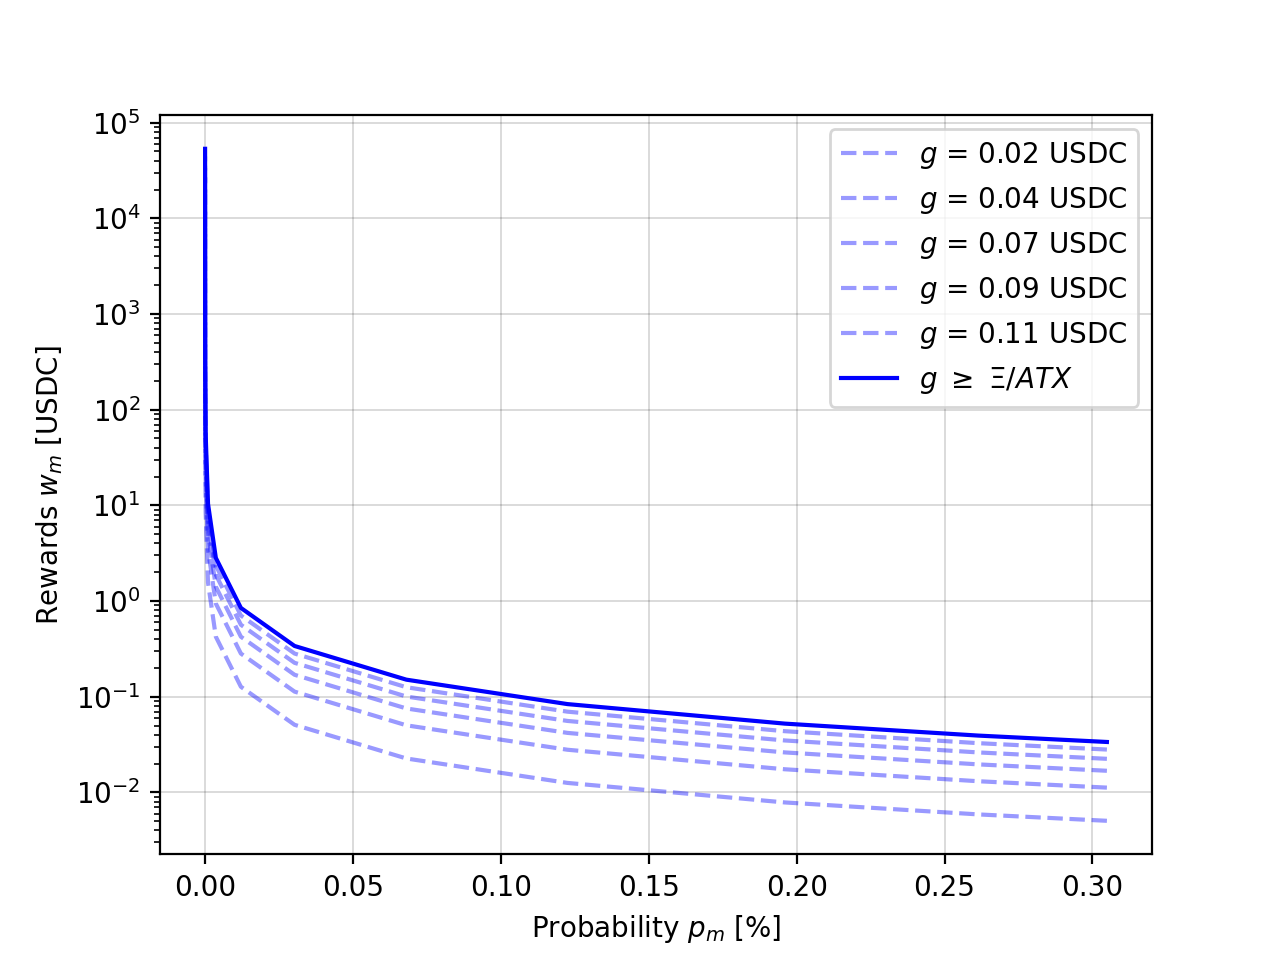
\includegraphics[width=1.1\linewidth]{images/trf4.png}
  \caption{y-log scale}
  \label{fig:sfig1}
\end{subfigure}%
\begin{subfigure}{.5\textwidth}
  \centering
  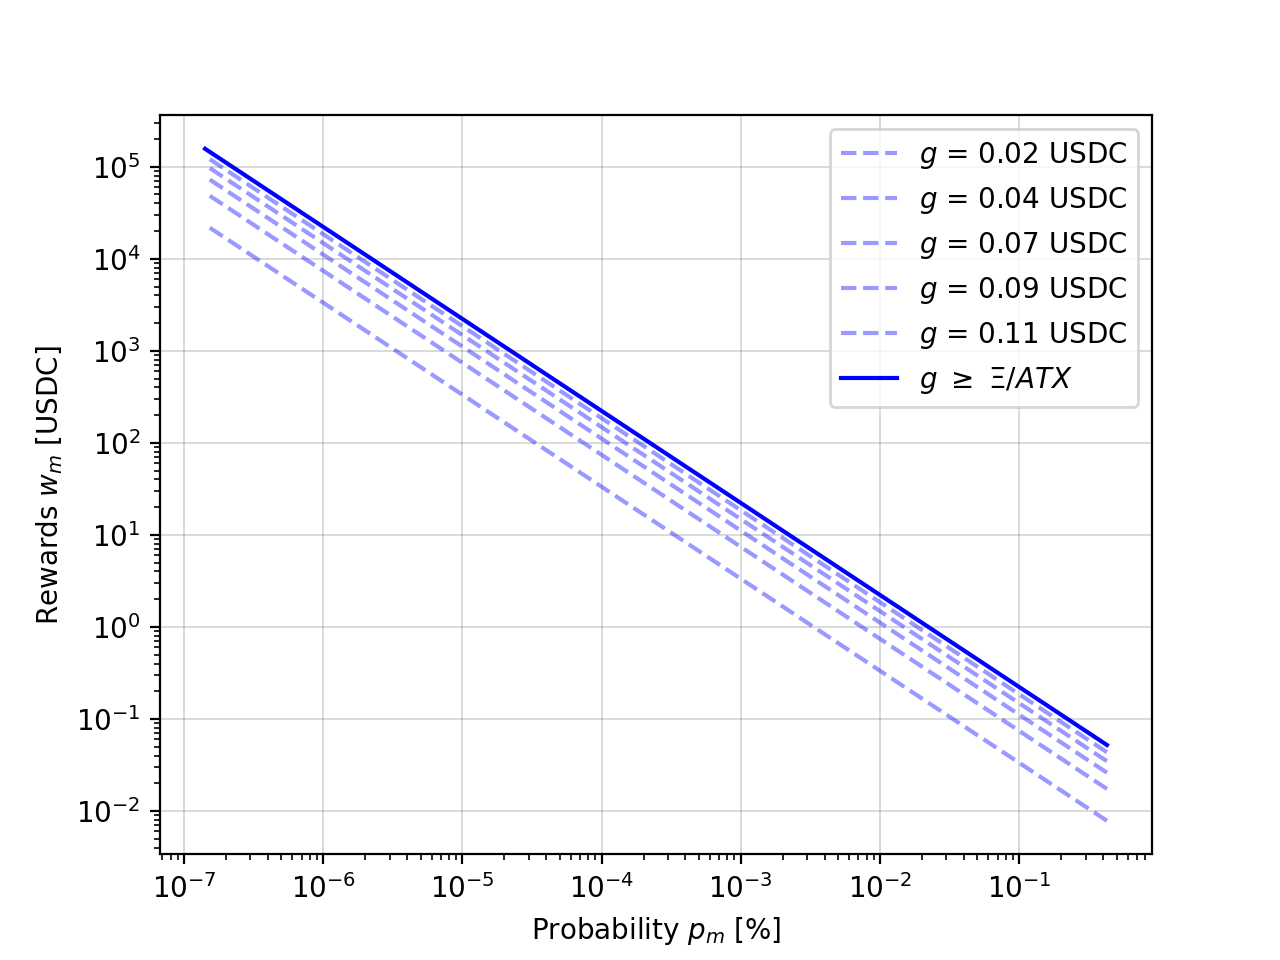
\includegraphics[width=1.1\linewidth]{images/trf3.png}
  \caption{log-log scale}
  \label{fig:sfig2}
\end{subfigure}
\caption{Plots of the TRF with the Optimistic Solution}
\label{fig:fig}
\end{figure}

\clearpage

\newpage


\section{Monetary Policy}
The Fluidity Protocol is governed through the Fluidity Governance Token. The Fluidity Governance Token facilitates voting on policies while identifying and aligning incentives for the long-term success of the protocol.

\subsection{Tokenomics}
The total supply of Fluid Governance tokens is 1,000,000,000 FLUID tokens, which will be fully circulating no earlier than 4 years post Token Generation Event (TGE.) The token distribution is as follows:

\vspace{1em}
 \begingroup
            \centering{
            \begin{tabular}{||c|c|c||}
            \hline
            \textit{Item} & \textit{Description} & \textit{Percentage} \\\hline
            Seed & Seed Round Investors & \ 13.0\% \\ \hline
            Private & Private Round Investors &\ 5.0\%\\ \hline
            Public & IDO/ IEO &\ 10.0\%\\ \hline
            Community & Utility Mining and Distribution &\ 20.0\%\\ \hline
            Retroactive & Reserved for Airdrops &\ 1.0\%\\ \hline
            DAO & Controlled by Token Holders &\ 26.0\%\\ \hline
            Foundation & Fluidity Foundation and Partners &\ 20.0\%\\ \hline
            Team &Current and Future Team Members&\ 5.0\%\\ \hline
            Sum & &\ 100.0\%\\ \hline

            \end{tabular}}
            \par
\endgroup
           \vspace{1em}

The token emission schedule is as follows:

\begin{figure}[h]
    \centering
    \includegraphics[width=12cm]{images/chart-1.png}
    \caption{Token Emission Schedule}
\end{figure}


\vspace{1em}

\newpage

The Fluidity token supply ownership evolves post-TGE like such:

\begin{figure}[h]
    \centering
    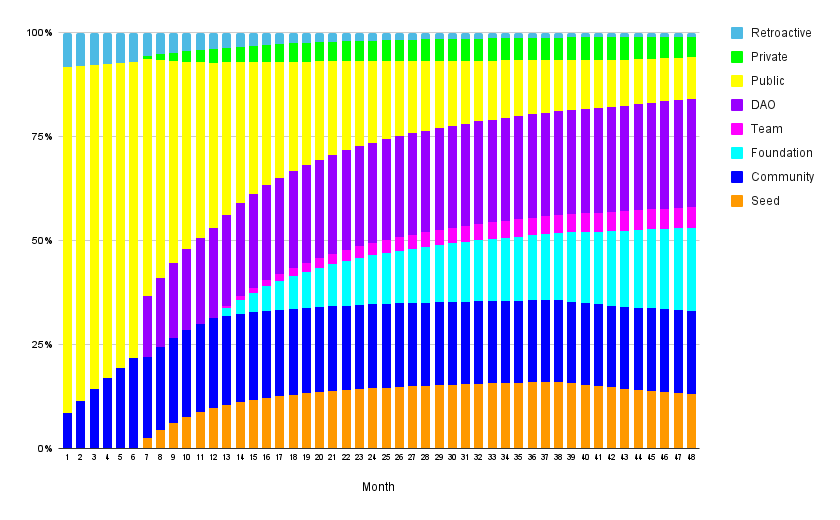
\includegraphics[width=12cm]{images/chart (18).png}
    \caption{Token Emission Schedule}
\end{figure}


\subsection{Token Emission Dilemma and Fluidity}

The objective of the governance token distribution is to maximise diversification amongst genuine users while incentivising positive value creation within the ecosystem. The development of the protocol must be funded and incentives need to be provided to stimulate long-term growth. Much of the funding required to build and grow the protocol, is received and given to a centralised and small number of entities. If these entities have the majority of the circulating supply of governance tokens, they may be able to vote on governance decisions that are favourable to their outcomes over the best interests of the wider ecosystem. Fluidity will minimise and control for this bad behaviour by distributing the majority of the float within the community using its novel Transfer Reward Function distribution.

\subsubsection{Float and Liquidity Mining}
A small float at TGE can inflate the price significantly early, benefiting early insiders. This is unsustainable and misaligns incentives for early token holders, as they will face significant inflation. The protocol faces a dilemma between early and quick growth by introducing a float, or the programmatic distribution of the tokens in a decentralised manner. Liquidity Mining is a method generally employed to increase the float and "hack" the growth of the protocol. Users can accumulate more coins as they enter circulation and actively increase their token holdings with inflation. Much of the liquidity provided in current liquidity mining programs is acquisitive liquidity, as the liquidity providers have no vested interest in the protocol.

 A bonus or lockup with a time multiplier effect can make liquidity more valuable to the protocol. One potential strategy is to introduce Vesting Schedules as a method to reduce selling pressure. However, this model can be improved upon - there is an argument to be made for rewarding active participation in the utility of a protocol, rather than passively participating through liquidity mining and vesting schedules.

Fluidity is exploring a custom model titled Utility Mining that behaves in a manner similar to growth hacking. Users are provided tokens for providing liquidity, but the tokens are vested in a programmatic manner emphasising utility as opposed to time. Utility is defined as the use of Fluid Assets. Liquidity providers will redeem their governance tokens as they use the protocol and engage with the ecosystem proportionate to the amount of liquidity they are providing.

\subsection{Fluidity Governance Token}

Governance is the core of the Fluidity Ecosystem as it provides guidance and structure on determining the size and frequency of payouts, the sources of yield and the token distribution policies. The governance token also entitles the holders to have an increased expected outcome overtime of receiving larger dividends when utilising their Fluid Assets.


\subsubsection{Utility Mining and Distribution}

Fluidity proposes a novel hybrid method to traditional Liquidity Mining programs titled Utility Mining. Although Liquidity Mining will still be utilised, a significant portion of the Fluidity governance tokens will be distributed through Utility Mining. Utility Mining utilises Fluidity's Transfer Reward Function, to provide a fairer mechanism for the distribution of governance tokens, incentivising proactive participation in the protocol and broader ecosystem.

Utility Mining rewards users with governance tokens and other incentives when they utilise the protocol for intended behaviours. In the Fluidity Protocol, a significant portion of the tokens in the float will be rewarded through utility mining. Utility Mining will ensure that many users understand the functionality and features of Fluidity as participation is necessitated to receive rewards.

\subsubsection{Liquidity as a second order effect of utility}

Utility Mining facilitates organic liquidity within the ecosystem. To participate in Utility Mining, a user must transact with a Fluid Asset. For one to participate in Utility Mining, there must be a liquidity provision event for that specific Fluid Asset. Although one can purchase a Fluid Asset on the open market, significant demand for Fluid Assets will cause a supply shock, only to be redeemed through an increase in minting Fluid Assets. This exchange will generate extra liquidity within the ecosystem. This generates a positive feedback loop, where an increase in the subsequent liquidity causes an increase in utility, as the reward pool grows.

\subsubsection{Broader Ecosystem Participation}
Fluidity increases the utility of assets in the broader ecosystem. By the creation of Fluid Assets, users are now incentivised to utilise their principal rather than holding it idle. By adding modifications to Fluidity's TRF, Fluidity can incentivise participation in value-add use-cases. This includes marketplaces, decentralised exchanges and any use-case where tokens are being transacted on chain. Utility Mining creates an incentive for users to participate in these very use-cases and aligns the communities with genuine participation within the protocol.

\subsubsection{Multiplier effect - Expected Outcome Farming}

As governance token holders have a higher stake in the Fluidity Ecosystem, Fluidity rewards them overtime with a higher Expected Outcome in the form of a multiplier, that increases the exposure to significantly larger dividends when they utilise Fluid assets. This increase in expected outcome can be quantified on a monetary value as it is directly tied to the size of the reward pool and exposure to a larger reward. Eventually Governance Token holders will be allowed to mint this increased Expected Outcome and sell it to speculators who may want to improve their exposure to larger dividends, and pay a premium to do so.

\subsubsection{Utility Orchestration}

Fluidity will incentivise users to participate in specific actions or protocols by rewarding them with a higher expected outcome of receiving a larger dividend payout. This has implications for chosen protocols as they will be receiving a significant gain in volume through Fluid Assets.

A potential outcome of this process is that when trading on DEX A, the expected outcome of receiving a larger payout is four times greater than DEX B. This increased expected outcome can cause a shift in volume of Fluid Assets DEX A for the next period. This shift is led by users seeking a higher expected outcome on a payout without a reduction in utility, as a rational user would aim to maximise their attached expected outcomes.
This can also have second order impacts, where Governance can incentivise more protocols and use cases to participate in Fluid Assets, by increasing their expected outcome, potentially causing significant increase in volume and traction.


\subsubsection{Payout based buyback and perpetual liquidity fund}


A proportion of each reward paid out will be utilised as a fee to contribute to the overall net-benefit of the protocol. As liquidity grows within Fluidity Protocol, the amount of dividends paid out will be increased, causing this fund to increase in size. The fund will be using approximately half of its funds buying back and burning the governance token. This will generate constant buying pressure on the governance token, creating supply scarcity and reduction in inflation introduced through Expected Outcome farming. The fund will also be utilising the rest of its money for perpetual liquidity on the protocol. This liquidity will never be moved unless in black swan scenarios including exploits resulting in loss of funds.


\newpage

\section*{Acknowledgements}

We would like to thank the RMIT Blockchain Hub\footnote{\url{https://rmitblockchain.io/}} for their review of this paper and their comprehensive feedback.

\newpage

\printbibliography

\end{document}
